En este experimentos queremos lograr el mismo comportamiento que tuvimos en el experimento [\ref{exp1}]. Haciendo un filtrado simple de los \emph{webaccess log } que hemos estado analizando podemos llegar a mejores valores que las predicciones de resultado aleatorio.





	\begin{figure}[t] 
		\centering
			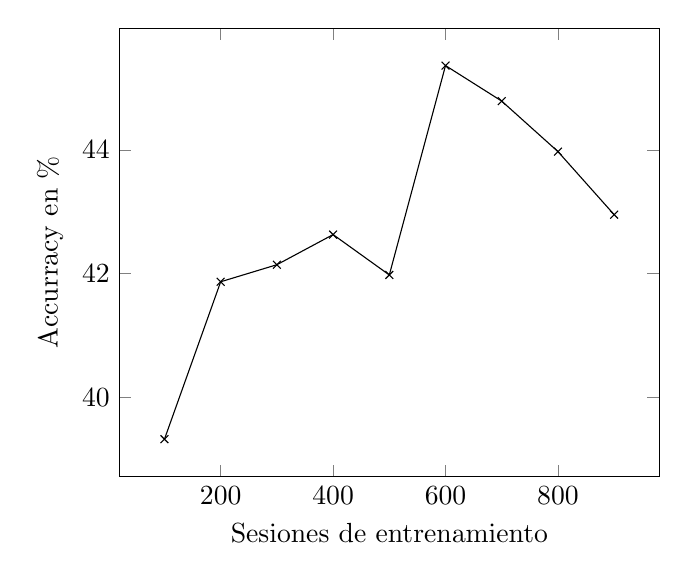
\begin{tikzpicture}
			\begin{axis}[
			xlabel=Sesiones de entrenamiento,
			ylabel=Accurracy en \% ]
			\addplot[color=black,mark=x] coordinates {
				(100, 39.3259176863181 )
				(200, 41.8698372966207 )
				(300, 42.1454458750596 )
				(400, 42.6323038397328 )
				(500, 41.9799599198396 )
				(600, 45.3634085213033 )
				(700, 44.7892976588628)
				(800, 43.9736180904522 )
				(900, 42.9539842873176 )
			};
			\end{axis}
			\end{tikzpicture}
		\caption{Gráfico de Accuracy vs sesiones de largo constante}
		\label{fig:sim}
	\end{figure}


\begin{table}[h] \label{my-label}
	\centering
	\resizebox{1\textwidth}{!}{
	\begin{tabular}{ccccc}
		\textbf{pruebas}     & \textbf{entrenamiento} & \textbf{accuracy}    & \textbf{nodos}       & \textbf{niveles}     \\
		800                  & 100                    & 0,203715239154616    & 150                  & 5                    \\
		700                  & 200                    & 0,212302878598247    & 150                  & 5                    \\
		600                  & 300                    & 0,226490224129709    & 300                  & 16                   \\
		500                  & 400                    & 0,243752086811352    & 1005                 & 48                   \\
		400                  & 500                    & 0,262308617234469    & 1005                 & 48                   \\
		300                  & 600                    & 0,258692564745196    & 1015                 & 48                   \\
		200                  & 700                    & 0,288423315814619    & 1023                 & 48                   \\
		100                  & 800                    & 0,28829431438127     & 1023                 & 48                   \\
		\multicolumn{1}{l}{} & \multicolumn{1}{l}{}   & \multicolumn{1}{l}{} & \multicolumn{1}{l}{} & \multicolumn{1}{l}{}
	\end{tabular}
	}
		\caption{Tabla resumen de experimento 3}
\end{table}

	
\begin{table}[]
	\centering \label{freq:exp3}
	\resizebox{1\textwidth}{!}{
	\begin{tabular}{lccccccccccccccccc}
		\textbf{símbolo}    & A   & B    & C   & D   & E   & F    & G   & H   & I   & J    & K   & L   & M   & N    & O  & P  & Q  \\
		\textbf{frecuencia} & 861 & 1502 & 509 & 412 & 557 & 1163 & 557 & 626 & 272 & 2252 & 399 & 703 & 301 & 1889 & 67 & 57 & 98
	\end{tabular}
	}
		\caption{Frecuencia de símbolos para experimentos con sesiones de largo constante.}	
	
\end{table}	
	
	
	La cantidad total de sesiones usadas fueron $1.000$ y las cuales como en el gráfico anterior se señala a mayor cantidad entrenamiento existe al menos un punto de la curva que se vuelve un máximo.


	Seguido a esto podemos ver el tiempo de construcción del \emph{trie} que nuestro modelo demora en generar:
	
	
	
	\begin{figure}[h] 
		\centering
		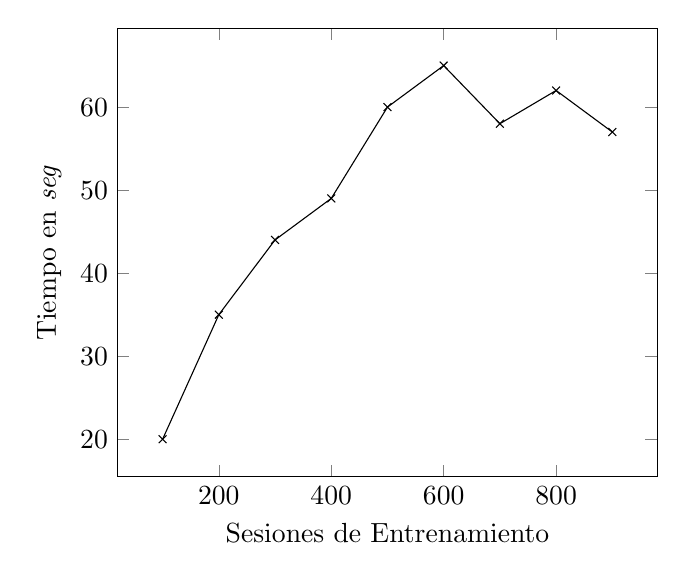
\begin{tikzpicture}
		\begin{axis}[
		xlabel= Sesiones de Entrenamiento ,
		ylabel=Tiempo en \emph{seg} ]
		\addplot[color=black,mark=x] coordinates {
			(100, 20)
			(200, 35)
			(300, 44)
			(400, 49)
			(500, 60)
			(600, 65)
			(700, 58)
			(800, 62)
			(900, 57 )
		};
		\end{axis}
		\end{tikzpicture}
		\caption{Gráfico de Tiempo vs sesiones de largo constante}
		\label{fig:sim}
	\end{figure}
	
	

	Al igual que en el gráfico anterior podemos ver que existe al menos una mínima cantidad sesiones las cuales generar un rendimiento sobre las evaluaciones a realizar. 